\section{软件设计}

\subsection{数据结构}

\subsubsection{Go Back N 协议}

\begin{lstlisting}[language=C,basicstyle=\tiny\sfmono]
#define DATA_TIMER 2000 // 重传计时器
#define ACK_TIMER 1100  // ACK计时器
#define MAX_SEQ 7       // 帧序号最大值
#define inc(k)                                                                 \
  if (k < MAX_SEQ)                                                             \
    k++;                                                                       \
  else                                                                         \
    k = 0;

typedef unsigned char frame_kind;      // 帧类型
typedef unsigned char seq_nr;          // 帧序号
typedef unsigned char packet[PKT_LEN]; // 数据包

typedef struct FRAME {  // 帧格式
  frame_kind kind;      // 帧类型
  seq_nr ack;           // ACK序号
  seq_nr seq;           // 帧序号
  packet info;          // 帧数据
  unsigned int padding; // CRC填充
} frame;
  
static int phl_ready = 0;        // 物理层状态
static unsigned char no_nak = 1; // ACK状态

static seq_nr next_frame_to_send;  // 发送窗口下一个发送
static seq_nr ack_expected;        // 发送窗口希望的ACK
static seq_nr frame_expected;      // 接收窗口希望的帧序号
static frame r;                    // 接受的帧
static packet buffer[MAX_SEQ + 1]; // 数据缓存
static seq_nr nbuffered;           // 已经缓存的帧数目
\end{lstlisting}

\subsubsection{选择重传协议}

\begin{lstlisting}[language=C,basicstyle=\tiny\sfmono]
#define DATA_TIMER 6000             // 重传计时器
#define ACK_TIMER 5100              // ACK计时器
#define MAX_SEQ 43                  // 帧序号最大值
#define NR_BUFS ((MAX_SEQ + 1) / 2) // 窗口大小
#define inc(k)                                                                 \
  if (k < MAX_SEQ)                                                             \
    k++;                                                                       \
  else                                                                         \
    k = 0;

typedef unsigned char frame_kind;      // 帧类型
typedef unsigned char seq_nr;          // 帧序号
typedef unsigned char packet[PKT_LEN]; // 数据包

typedef struct FRAME {  // 帧格式
  frame_kind kind;      // 帧类型
  seq_nr ack;           // ACK序号
  seq_nr seq;           // 帧序号
  packet info;          // 帧数据
  unsigned int padding; // CRC填充
} frame;

static int phl_ready = 0;        // 物理层状态
static unsigned char no_nak = 1; // ACK状态

static seq_nr next_frame_to_send; // 发送窗口下一个发送
static seq_nr ack_expected;       // 发送窗口希望的ACK
static seq_nr frame_expected;     // 接收窗口希望的帧序号
static seq_nr too_far;            // 接收窗口右端点的下一个
static frame r;                   // 接收的帧
static packet in_buf[NR_BUFS];    // 接收窗口缓冲
static packet out_buf[NR_BUFS];   // 发送窗口缓冲
static bool arrived[NR_BUFS];     // 记录完成的帧
static seq_nr nbuffered;          // 已经缓存的帧数目
\end{lstlisting}

\subsection{模块结构}

\begin{lstlisting}[language=C,basicstyle=\tiny\sfmono]
/*
 * 判断某个序号是否在窗口内
 * a 左下标
 * b 判断的值
 * c 右下标的下一个
 */
static unsigned char between(seq_nr a, seq_nr b, seq_nr c) {
  return ((a <= b && b < c) || (c < a && b < c) || (c < a && a <= b));
}

/*
 * 发送帧添加校验位给物理层
 */
static void put_frame(unsigned char *frame, int len) {
  *(unsigned int *)(frame + len) = crc32(frame, len);
  send_frame(frame, len + 4);
  phl_ready = 0;
}

/*
 * 填充内容发送给物理层
 */

static void send_data_frame(frame_kind fk, seq_nr frame_nr,
                            seq_nr frame_expected, packet buffer[]) {
  frame s;
  s.kind = fk;
  s.ack = (frame_expected + MAX_SEQ) % (MAX_SEQ + 1);
  stop_ack_timer();

  if (fk == FRAME_DATA) {
    s.seq = frame_nr;
    memcpy(s.info, buffer[frame_nr % NR_BUFS], PKT_LEN);
    dbg_frame("Send DATA %d %d, ID %d\n", s.seq, s.ack, *(short *)s.info);
    put_frame((unsigned char *)&s, 3 + PKT_LEN);
    start_timer(frame_nr, DATA_TIMER);
  } else if (fk == FRAME_ACK) {
    dbg_frame("Send ACK  %d\n", s.ack);
    put_frame((unsigned char *)&s, 2);
  } else if (fk == FRAME_NAK) {
    dbg_frame("Send NAK  %d\n", (s.ack + 1) % (MAX_SEQ + 1));
    no_nak = 0;
    put_frame((unsigned char *)&s, 2);
  }
}
\end{lstlisting}


\subsection{算法流程}

\begin{figure}[h]
  \centering
  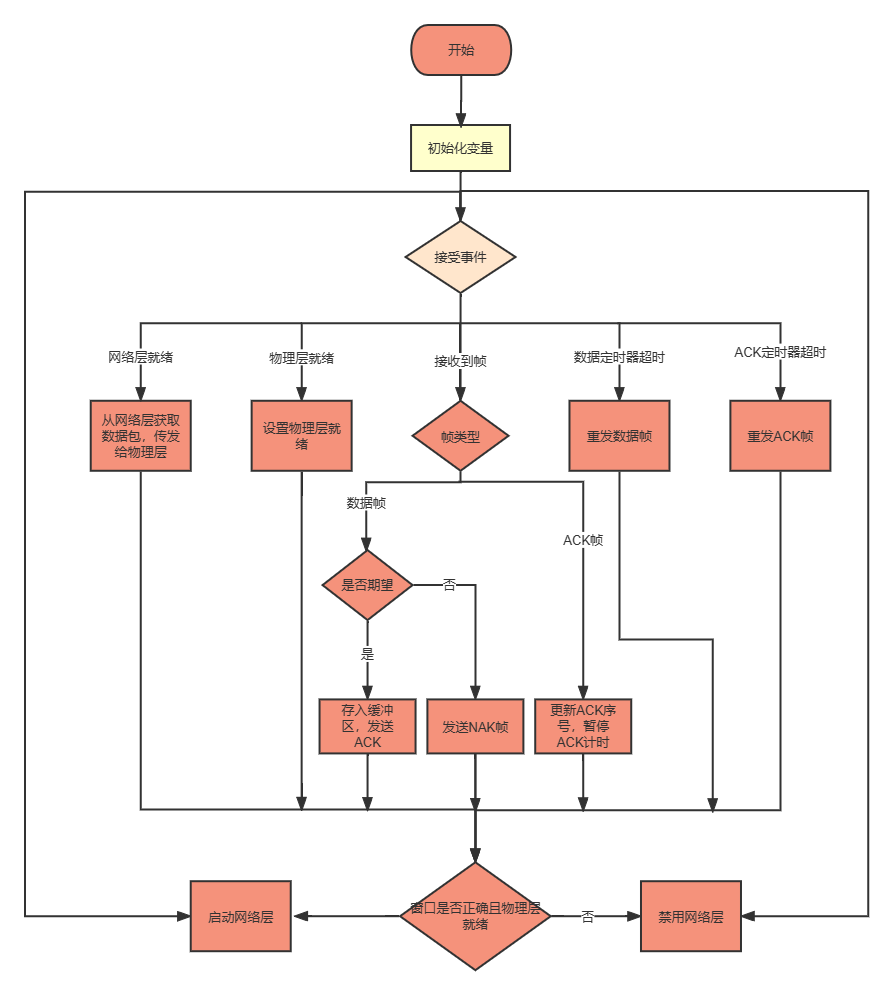
\includegraphics[width=1\textwidth]{figure/process.png}
  % \caption*{数据结果记录表}
  \label{fig:process}
\end{figure}